\section{Introduction and Motivation}


\subsection{Problem of Interest}
%%%%%%%%%%%%%%%%%%%%%%%%%%%%%%%%%%%%%%%%%%%%%%%%%%%%%%%%%%%%%%%%%%%%%%%%%%%%%%%%%%%%%%%%
\begin{frame}
	\frametitle{Multigroup Neutron Transport Equation (NTE) with Feedback}
	\vspace{-2em}
	\begin{equation}
	    \begin{aligned}
             \bW \cdot \nabla\psi_g(\br, \bW ) + \Sigma_{t,g}(\br,T) \psi_g(\br, \bW ) &=\lambda \frac{\chi_g(\br)}{4\pi} \sumgp \nu \Sigma_{f,g'}(\br,T) \phi_{g'}(\br)\\[-11pt]
           &+ \sumgp \int_{4\pi}\Sigma_{s,g'\to g}(\br,\bWp\to \bW,T)  \psi_{g'}(\br,\bWp) d\W    \label{eqn:transport}
        \end{aligned}
    \end{equation}
    \vspace{-2em}
    \begin{equation}
        \int dV\sumg\int_{4\pi}\Sigma_f\kappa\psi_g d\W=P\label{eqn:normalization}
    \end{equation}
    \vspace{-2em}
    \begin{equation}
        \boldsymbol{L}(T)T(\br)=\sumg\Sigma_{f,g}(\br,T)\kappa\Phi_g(\br)\label{eqn:th}
    \end{equation}
    \vspace{-2em}
	\begin{itemize}
	\item The smallest $\lambda \equiv \frac{1}{k}$ eigenvalue, its corresponding eigenvector $\psi$, and the associated temperature distribution $T$ are desired from this set of coupled equations.
	\vspace{-0.5em}
	\item A normalization condition must be imposed to ensure a unique solution to the transport eigenvalue problem.
	\vspace{-0.5em}
	\end{itemize}
	\vfill
\end{frame}
%%%%%%%%%%%%%%%%%%%%%%%%%%%%%%%%%%%%%%%%%%%%%%%%%%%%%%%%%%%
\begin{frame}
\frametitle{Overall Iteration Schemes}

\vspace{-0.5em}
\begin{itemize}
    \item Iteration Scheme:
    \begin{itemize}
        \item \textbf{Picard}
        \vspace{-0.5em}
        \item Each Physics is solved separately
        \vspace{-0.5em}
        \item Easy to implement
    \end{itemize}
    \vspace{-0.2em}
    \item Transport iteration Scheme:
     \begin{itemize}
         \item Source Iteration
         \vspace{-0.5em}
         \item Iterates on eigenvalue, and scattering \\
         and fission sources
         \vspace{-0.5em}
         \item Converges very slow
     \end{itemize}
     \vspace{-0.2em}
    \item Acceleration Scheme:
    \begin{itemize}
        \item \textbf{Nonlinear Diffusion Acceleration (NDA)}
        \vspace{-0.5em}
        \item Reduce the total outer iteration number by orders of magnitude
    \end{itemize}
    \vspace{-0.2em}
    \item Eigenvalue Solver:
    \begin{itemize}
        \item Wielandt Shifted Power Iteration
    \end{itemize}
\end{itemize}
  \begin{picture}(5,5)
     \put(230,70){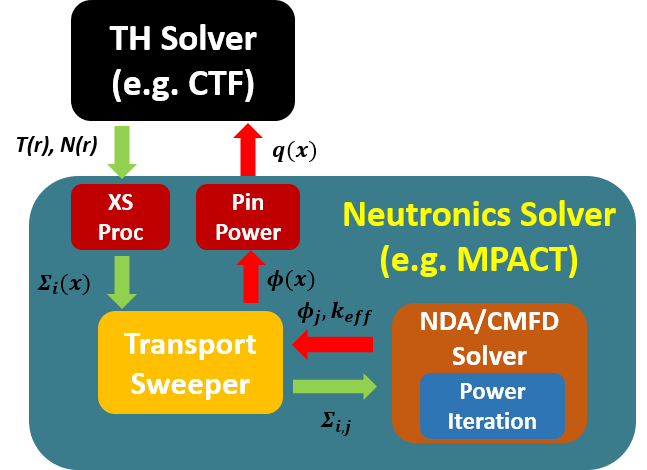
\includegraphics[width=0.45\textwidth]{Texfile/Figure/Picard.png}}
  \end{picture}
\end{frame}
%%%%%%%%%%%%%%%%%%%%%%%%%%%%%%%%%%%%%%%%%%%%%%%%%%%%%%%%%%%%%%%%%%%%%%%%%%%%%%%%%%%%%%%%%%%%%%
\begin{frame}
    \frametitle{Nonlinear Diffusion Acceleration, Coarse Mesh Finite Difference}
    \begin{itemize}
        \item Nonlinear Diffusion Acceleration (NDA) is a common acceleration method employed by the nuclear reactor community:
            \begin{itemize}
                \item Low-order, transport-corrected diffusion equation
                \vspace{-0.5em}
                \item Nonlinear correction term $\hat{D}$ obtained from a high-order transport sweep
                \vspace{-0.5em}
			    \item Scalar flux and eigenvalue solution used as an improved estimate for the scattering and fission source terms in a subsequent transport sweep
            \end{itemize}
    \end{itemize}
    \vspace{-0.25cm}
	\begin{equation}
	  \begin{aligned}
	    &\l[-\nabla \cdot D_g(\br,T) \nabla + \Sigma_{t,g}(\br,T)+\hat{D}_g(\br,T) \r] \phi_g(\br) =\\[-13pt]
	    &\hspace{4cm}\sumgp \Sigma_{s0,g' \to g} (\br,T) \phi_{g'}(\br) + \lambda \chi_g(\br) \sumgp \nu \Sigma_{f,g'}(\br,T) \phi_{g'}(\br) \end{aligned}\label{eqn:eig}
	\end{equation}\\[-1em]
	\begin{itemize}
	    \item Coarse Mesh Finite Difference (CMFD) : a generalization of NDA which allows for a coarser mesh to be used on the low-order problem
	\end{itemize}	
\end{frame}
%%%%%%%%%%%%%%%%%%%%%%%%%%%%%%%%%%%%%%%%%%%%%%%%%%%%%%%%%%%%%%%%%%%%%%%%%%%%%%%%%%%%%%%%
\begin{frame}
	\frametitle{ Wielandt-Shifted Power Iteration}
	\begin{itemize}
	    \item Martix form of \refeqn{eig}:
	    \begin{equation}
	        \mathbf{M\phi}=\lambda\mathbf{F}\phi
	    \end{equation}
	    \vspace{-1.5em}
		\item Standard power iteration (PI):
				\begin{gather}
					\mathbf{M} {\bphi}^{(l+1)} = \lambda^{(l)} \mathbf{F}  \bphi^{(l)}  \\
					\lambda^{(l+1)} = \lambda^{(l)} \| \mathbf{F} \bphi^{(l)}\|/\| \mathbf{F} \bphi^{(l+1)}\|
				\end{gather}
		PI converges at a rate equal to the dominance ratio (DR): $\lambda_1/\lambda_2$
		\vspace{-0.3em}
		\item Because the DR is close to 1 for realistic reactor problems, we can improve the spectral radius of PI using a Wielandt Shift (WS):
			\begin{equation}
				\l[ \mathbf{M} - \lambda_s\mathbf{F} \r] \bphi^{(l+1)} = \l[ \lambda^{(l)} - \lambda_s \r] \mathbf{F}  \bphi^{(l)} \label{eqn:WS}
			\end{equation}
		\item In practice, this ``inner'' iteration procedure is not full converged, instead it is truncated at a given total number of iterations $L$ or when some other convergence criteria is met
	\end{itemize}
\end{frame}

\subsection{Motivation}
%%%%%%%%%%%%%%%%%%%%%%%%%%%%%%%%%%%%%%%%%%%%%%%%%%%%%%%%%%%%%%%%%%%%%%%%%%%%%%%%%%%%%%%%
\begin{frame}
\vspace{-1.5em}
\frametitle{Picard iteration scheme is more stable than we have expected}
\tikzmark{mybox}{}
\begin{itemize}
\item Drawbacks of the Picard scheme:\\[0.2em]
\begin{itemize}
    \item Stability is not guaranteed
    \vspace{-0.5em}
    \item Relaxation is always used
\end{itemize}
\vspace{-0.5em}
\item Furthermore, Theoretical Analysis~\footfullcite{Kochunas2017FourierSections}:\\[0.2em]
\begin{itemize}
    \item Relaxation could not help \\
    when $\Sigma_tX>100$
    \vspace{-0.5em}
    \item Hmm, the optical thickness of a 3D \\
    pincell is around 100.
\end{itemize}
\vspace{2em}
\item But, the multiphysics simulations have been performed for full core problems\\[0.2em].

\end{itemize}
    \begin{picture}(5,5)
     \put(220,35){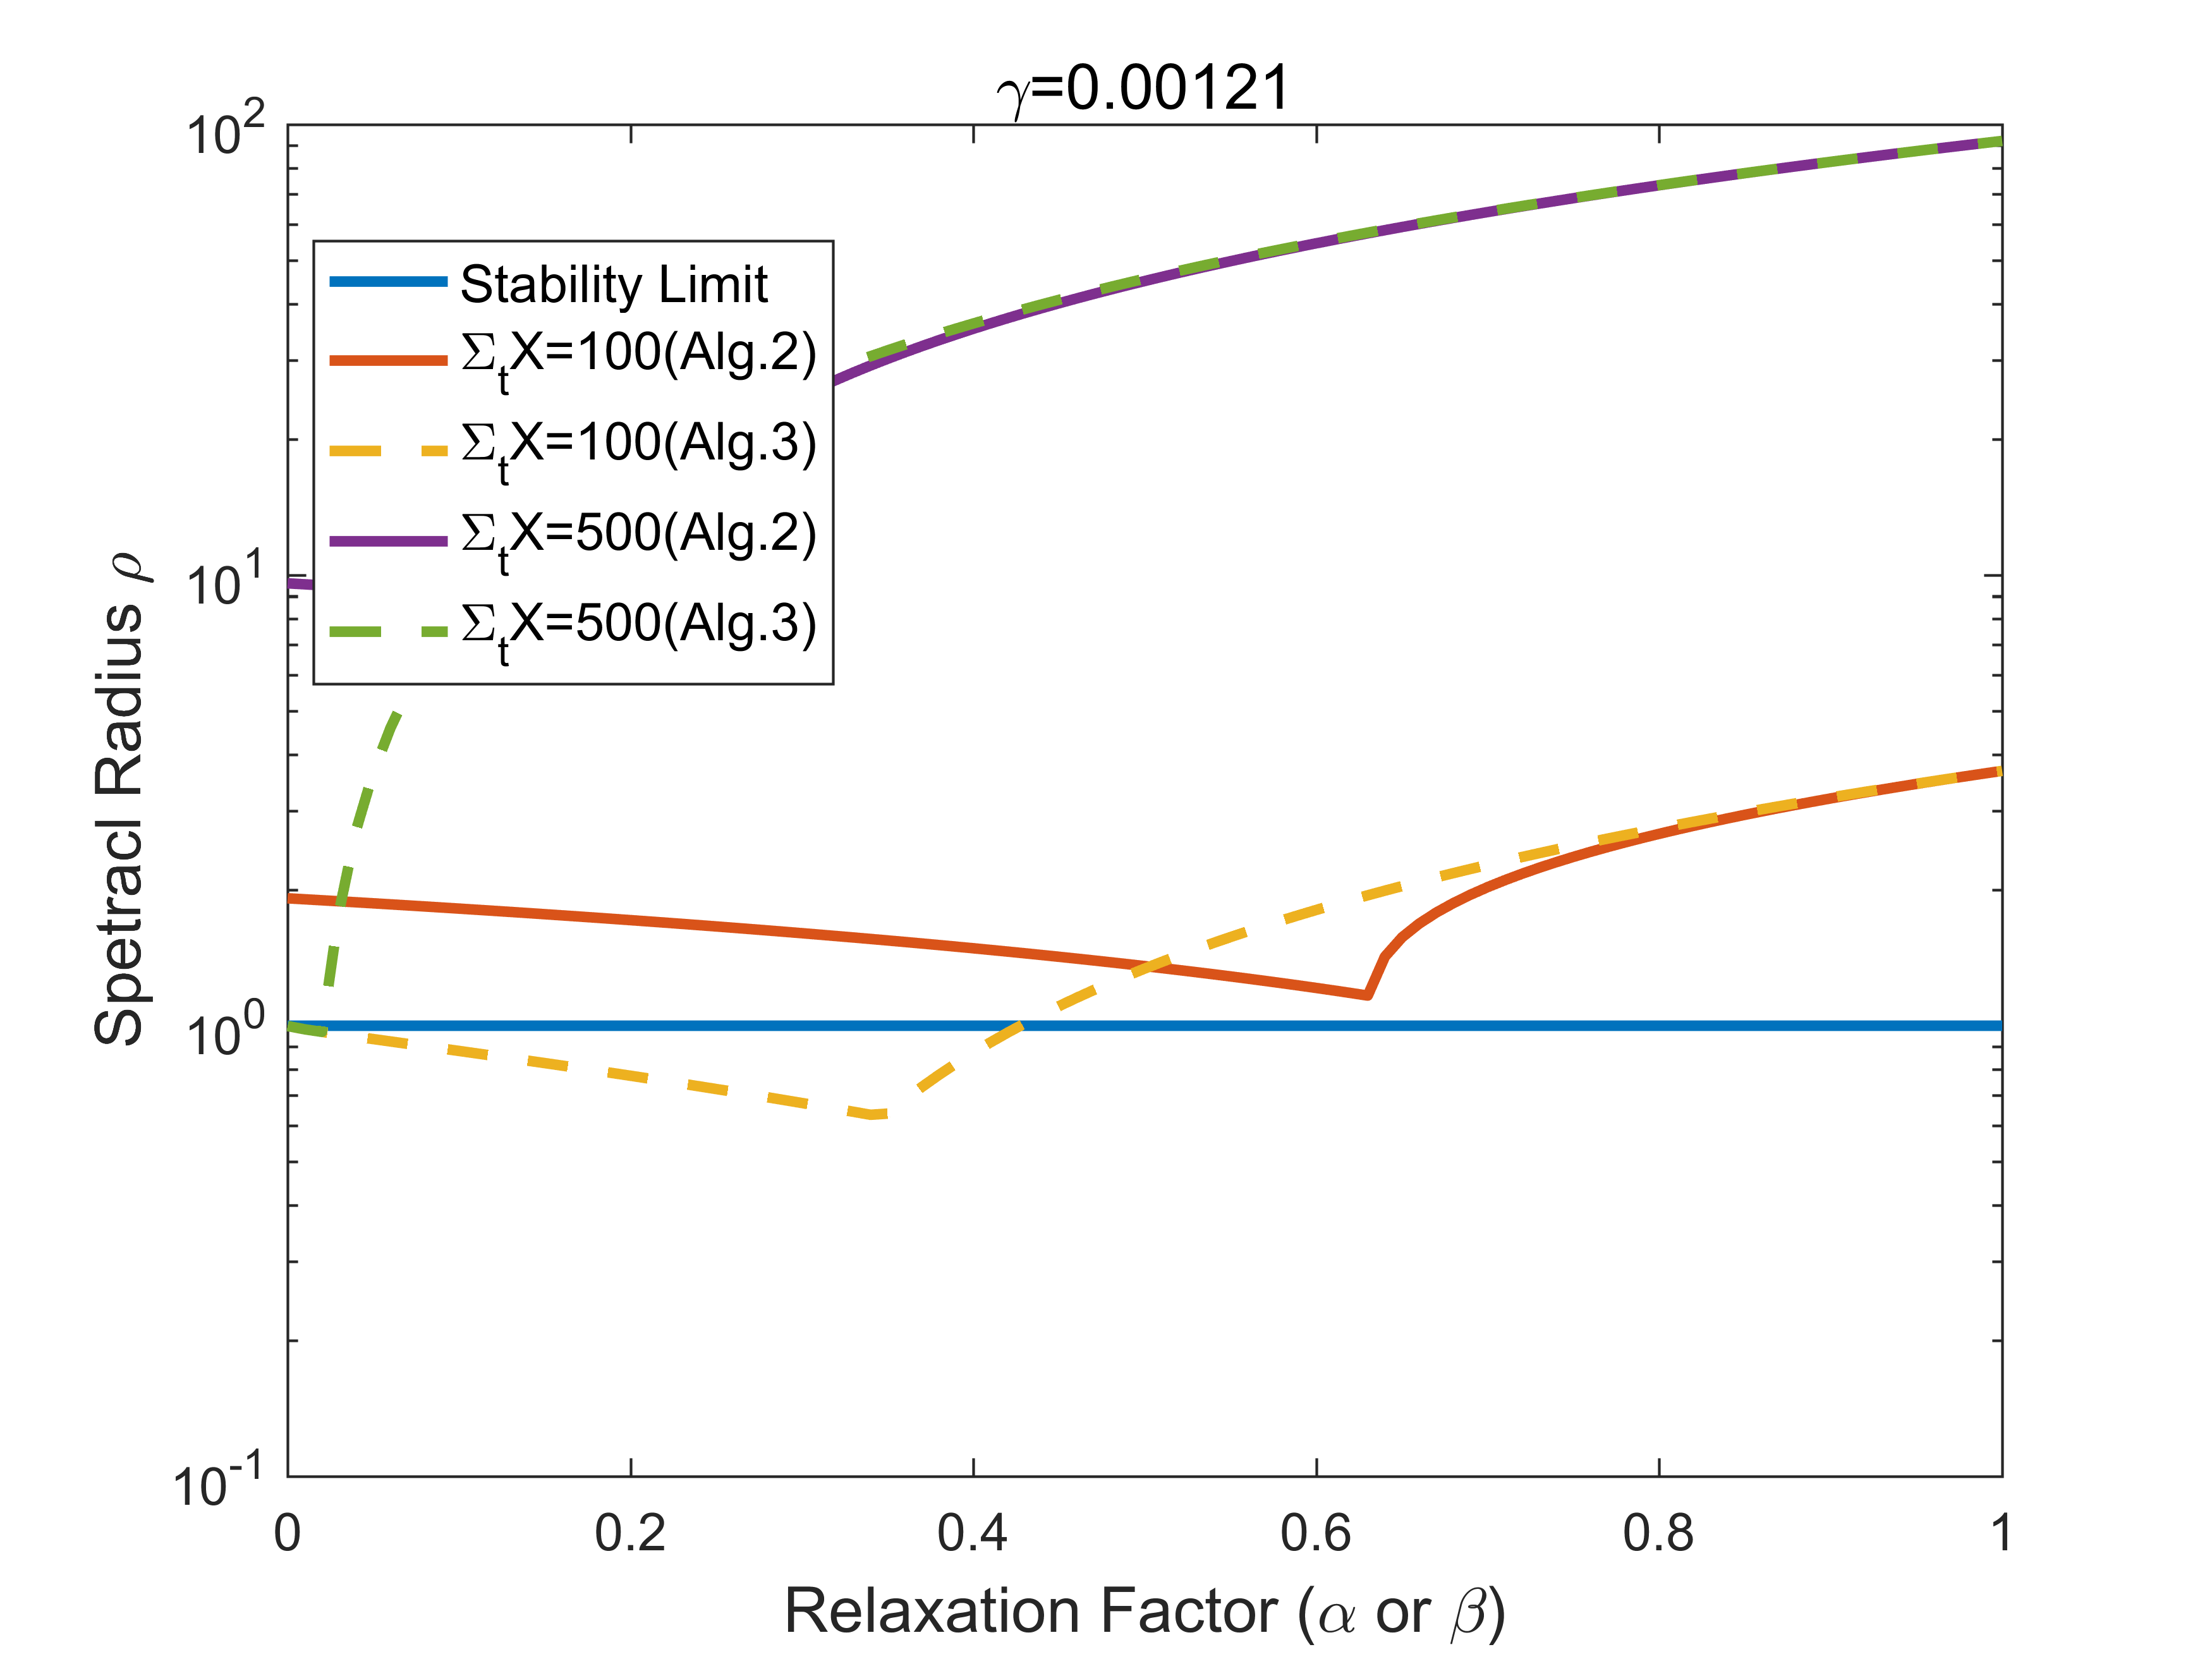
\includegraphics[width=0.45\textwidth]{Texfile/Figure/rhovalpha_old.png}}
  \end{picture}
%   \tikz[overlay,remember picture]{\draw[draw=red,thick,fill opacity=0] ($(mybox)+(1,-1)$) rectangle ($(mybox)+(8,-3.5)$);}
\vspace{-0.5em}
 \end{frame}


%%%%%%%%%%%%%%%%%%%%%%%%%%%%%%%%%%%%%%%%%%%%%%%%%%%%%%%%%%%%%%%%%%%%%%%%%%%%%%%%%%%%%%%%
\begin{frame} \frametitle{More accurate CMFD solutions make iterations scheme unstable}
\begin{enumerate}
    \item Example 1--3D Pin Cell
    \begin{itemize}
        \item Length: 380 $cm$, Power: 71 $kW$
        \vspace{-0.5em}
        \item $L$: $\#$ of power iteration, $nOuter$: $\#$ of total outer iteration
    \end{itemize}
    \begin{table} [!hbt]
    \centering
     \small
    \begin{tabular}{c|c|c|c|c|c|c|c|c} 
        \toprule
        \textbf{$L$}&2 & 4 & 6 & 10 & 15 & 20 &30&100\\ 
         \toprule
       \textbf{nOuter}&33&19&15&14&14&17&21&\textbf{N/A}\\
        \toprule
    \end{tabular}
    \end{table}
    \vspace{-1em}
    \item Example 2--Vera Problem 7
    \begin{table}[ht!]
        \centering
	\begin{tabular}{ccc}
    \toprule
        Method & nOuter & Total Runtime [s]  \\
        \midrule
   			Default & 15 &  10230 \\
  			MSED~\footfullcite{yee2019multilevel} & 20 &  9749 \\
  			MSED-L&  12  & 6057 \\
        \bottomrule
    \end{tabular}
    \begin{itemize}
        \item MSED-L:  A partially converged low order MSED solve with looser convergence criteria and less aggressive Wielandt shift
    \end{itemize}
\end{table}  
\end{enumerate}
\end{frame}
%%%%%%%%%%%%%%%%%%%%%%%%
%%%%%%%%%%%%%%%%%%%%%%%%%%%%%%%%%%%%%%%%%%%%%%%%%%%%%%%%%%%%%%%%%%%%%%%%%%%%%%%%%%%%%%%%%%
\begin{frame}{Goal of Research }
\vspace{-1em}
\begin{itemize}
\item \textbf{Questions to be answered}:
\begin{itemize}
    \item Can the effect of convergence of NDA (CMFD) be theoretically investigated?
    \begin{itemize}
        \item Previous researches on the stability of transport method always assume that NDA (CMFD) is fully converged.
    \end{itemize}
    \vspace{-0.5em}
    \item What is the relation between partial convergence and well-known relaxation?
        \begin{itemize}
            \item Effect of partial convergence is similar with the effect of relaxation
        \end{itemize}
    \item Whether the formula to determine near-optimal partial convergence can be derived?
        \begin{itemize}
            \item An near-optimal partial convergence seems to exist
            \vspace{-0.5em}
            \item Reduce the computational intensity-- \it{``why waste effort converging the low order problem with the wrong coefficients``}
            \vspace{-0.5em}
            \item Stabilize the iteration scheme
        \end{itemize}
\end{itemize}
\item Investigation Approach: \textbf{Fourier Analysis}
\end{itemize}
\vfill
\end{frame}
